% This sample file is dedicated to the public domain.
\chapter{Introduction}
\label{c.intro}

This thesis examines the design of robust and efficient distributed
database systems.

Over the past decade, the challenges of distributed systems design
have become increasingly mainstream. The rise of new application
domains such as Internet services and the continued decrease of
storage and computing costs have led to massive increases in request
and data volumes. To address these trends, application developers have
frequently turned to distributed systems designs. Scale-out
application programming frameworks, data serving systems, and data
processing platforms enjoy unprecedented popularity
today~\cite{mohan-note,queue,fnt-mr}. Coupled with the introduction of
inexpensive and elastic cloud computing~\cite{berkeley-view}, these
factors have led distribution and replication to become common
features in modern application and system designs. As a result, a
growing class of software must address the difficulties of robust
operation over computer networks, which include communication delays,
partial failures, and inherent uncertainty about global system
state~\cite{fallacies-deutsch}.

In many applications, the difficulties of distributed systems design
are relegated to a database tier. Application development best
practices delegate the management of application state to a database
back-end: application programmers implement application logic, while a
back-end data infrastructure system handles data storage, query
processing, and concurrency control~\cite{tamer-book}. This separation
of concerns means database systems frequently act as the keystone of
reliable distributed applications (Figure~\ref{fig:servers}). Thus,
database systems must directly address the challenges of distribution,
replication, and fault tolerance---while providing a user-friendly
interface for application developers and end users.


\begin{figure}[t!]
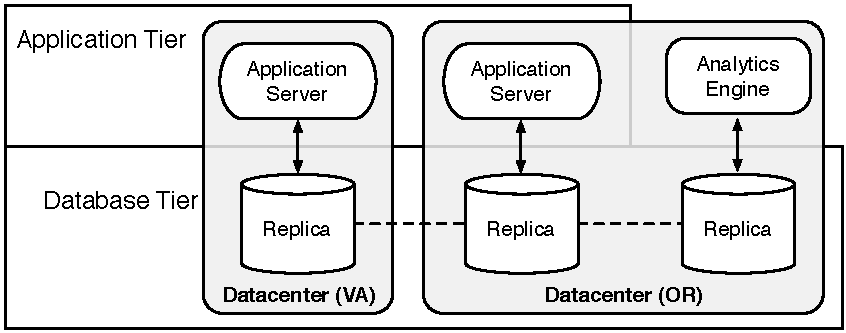
\includegraphics[width=\figscale\columnwidth]{diagram/servers.pdf}
\vspace{.5em}
\caption{An illustration of a distributed, replicated database and its
  relation to application servers and end users. In modern distributed
  databases, data is stored on several servers that may be located in
  geographically distant regions (e.g., Virginia and Oregon, or even
  different continents) and may be accessed by multiple database
  clients (e.g., application servers, analytics frameworks, database
  administrators) simultaneously. The key challenge that we
  investigate in this thesis is how to minimize the amount of
  synchronous communication across databases while providing ``always
  on,'' scalable, and high performance access to each replica.}
\label{fig:servers}
\end{figure}

In this work, we investigate a conceptually simple class of designs
for robust distributed databases: we study the design of databases
that allow applications to make non-trivial progress independent of
network behavior. That is, we study the design of database systems
that provide \textit{coordination-free} execution: whenever database
clients can access at least one copy of database state, they are
guaranteed to make non-trivial progress. This means that, in the
presence of communication failures between servers, each client's
operations may still proceed, providing ``always on'' functionality,
or guaranteed \textit{availability}. Even when database servers are
able to communicate with one another, communication is not
required. This allows \textit{low latency} operation: each client's
requests can be processed using locally accessible resources. Finally,
coordination-free execution ensures \textit{scalability}: as more
servers are added, the database can make use of them without
disrupting existing servers. This results in increased capacity. Thus,
coordination-free execution offers attractive performance and
availability benefits while ensuring that, subject to the availability
of additional resources, additional requests can be serviced on
demand.

This coordination-free database system design represents a departure from
classic database system designs. Traditionally, database systems
exposed a \textit{serializable transaction} interface: if user
operations are bundled into transactions, or groups of multiple
operations over multiple data items, a database providing
\textit{serializability} guarantees that the result of executing the
transactions is equivalent to some serial execution of the
transactions~\cite{bernstein-book}. Serializability is remarkably
convenient for programmers, who do not need to reason about
concurrency or distribution. However, serializability is inconvenient
for databases: serializability (provably) requires
coordination~\cite{davidson-survey}, negating the benefits of
coordination-free execution. Intuitively, enforcing a serial ordering
between transactions precludes the ability to guarantee
the transactions' independent progress when executed on multiple
servers.

As a result, increased application demands for availability, low
latency, and scalability have led to a recent schism within mainstream
database system designs~\cite{marcus-talk,mohan-note}.  A
proliferation of database systems, often called ``NoSQL'' systems,
forego serializability (and other ``strong'' semantics) in order to
provide coordination-free execution. However, in turn, these NoSQL
systems provide few, if any semantic guarantees about their query
results and about database state (also called \textit{safety
  properties}; e.g., ``no two users share a
username'')~\cite{queue,bernstein-survey,lamport-safety}. In contrast
with serializability, which guarantees that safety properties
preserved by individual transactions will be preserved under their
serial composition, these NoSQL stores leave the enforcement of
application safety to the application---a challenging and error-prone
proposition~\cite{consistency-borders,entitygroup}. Thus, database users and application programmers today
are left with one of two options: ensure safety via serializability
and coordination, or forego safety within the database but enjoy the benefits of
coordination-free execution.

In this thesis, we examine this apparent tension between ensuring
application safety properties within the database and enjoying the
scalability, availability, and performance benefits of
coordination-free execution. Is enforcing safety properties always at
odds with coordination-free execution? If we rely on serializability,
the answer is yes. Instead, we consider an alternative: the
enforcement of non-serializable semantic guarantees in a
coordination-free manner. By examining the safety properties of
today's database-backed applications, we determine whether
coordination is strictly necessary to enforce them and explore
implementations that limit the use of coordination. Thus, this thesis
explores the relationship between correctness---according to useful
safety guarantees---and coordination. More precisely, what is the
coordination cost of a given safety guarantee? What is the minimum
communication we must perform to enforce various correctness criteria?

\section{Coordination Avoidance}

Our primary goal in this thesis is to build database systems that
coordinate only when strictly required in order to guarantee
application safety. To realize this goal, we examine which semantic
guarantees databases \textit{can} provide under coordination-free
execution---and explore implementations that fulfill this
potential. We study a range of guarantees from both classic database
systems as well as guarantees required by modern database-backed
applications. Today, most of these guarantees are either implemented
using coordination or are not provided by coordination-free
systems. However, we demonstrate that many of these requirements can
be correctly implemented without coordination and provide algorithms
and system implementations for doing so. This enables what we call
\textit{coordination avoidance}: the use of as little coordination as
possible while maintaining safety guarantees on behalf of database
users.

\vspace{0.5em}
\noindent\textbf{Thesis Statement:} \textit{Many semantic requirements
  of database-backed applications can be efficiently enforced without
  coordination, thus improving scalability, latency, and
  availability.}

To achieve this goal, we first develop a new, general rule for
determining whether a coordination-free implementation of a given
safety property exists, called \textit{\iconfluence}. Informally,
\iconfluence determines whether the result of executing operations on
independent copies of data can be combined (or ``merged'') into a
single, coherent (i.e., \textit{convergent}) copy of database
state. Given a set of operations, a safety property that we wish to
maintain over all copies of database state, and a merge function,
\iconfluence tells us whether coordination-free execution is
possible. \Iconfluence is both necessary and sufficient: if
\iconfluence holds, a coordination-free, convergent implementation
exists. If \iconfluence does not hold, no system can implement the
semantics while also providing coordination-free, convergent
execution.

Given this \iconfluence criterion, we examine a set of common semantic
guarantees found in database systems and database-backed applications
today to determine whether a coordination-free execution strategy for
enforcing them exists. We perform several case studies, which we
describe in detail below. In many cases, although existing
implementations of these guarantees may rely on coordination, we show
that coordination-free implementations of the semantics exist. This
provides the scalability, performance, and availability benefits of
coordination-free execution---but without compromising desirable
semantic guarantees. None of these guarantees is serializable, but all
of them correspond to existing or emerging demands from
applications today.

Our use of \iconfluence recognizes latent potential for
coordination-free execution in existing and emerging applications. In
demonstrating this potential, we highlight a need for conscientious
consideration of coordination in the design of database systems: in
many \iconfluent scenarios, traditional and/or legacy implementations
designed for non-distributed environments over-coordinate and fail to
capture the potential for coordination-free execution. Conversely,
when \iconfluence does not hold, understanding when a
coordination-free implementation does not exist spares system
designers the effort of searching for a more efficient implementation
when in fact such an implementation does not exist.

Of course, simply recognizing that a coordination-free implementation
exists does not by itself lead to coordination-free systems. Rather,
we must also find a coordination-free implementation of \iconfluent
semantics. Therefore, we present the design, implementation, and
evaluation of several sets of \iconfluent guarantees. We demonstrate
order-of-magnitude improvements in latency and throughput over
traditional algorithms, validating the power of coordination-free
systems design. In addition to these case studies, we also present
more general design principles for realizing coordination avoidance in
practice. We note the importance of separating visibility from
progress, ensuring composability of operations, and controlling
visibility via multiversioning.

\minihead{By example} As a simple example, consider the common Read
Committed (RC) isolation guarantee~\cite{adya}, which is the default
semantics in fifteen of eighteen popular relational databases,
including Oracle, SAP Hana, and Microsoft SQL Server
(Chapter~\ref{c.isolation}). Informally, Read Committed ensures that
users never read non-final writes to data; if, within a transaction, a
user sets her username to ``Sally'' and, subsequently, sets her
username to ``Sal,'' no other user should ever read that the user's
username is ``Sally.'' The classic strategy for implementing Read
Committed isolation dates to the 1970s and relies on locking: when our
user wants to update her username record, she acquires a mutually
exclusive lock on the record~\cite{gray-isolation}. This is a
reasonable strategy for a single-node database, but the coordination
required to implement this mutual exclusion can be disastrous in a
modern distributed environment: while our first user holds the lock on
her username record, all other users who wish to also access the same
username record must wait.

While coordination is sufficient to enforce RC isolation (via
locking), is it strictly necessary? We can apply the principle of
\iconfluence here: informally, if each individual user never observes
non-final writes (i.e., each individual read-write history is valid
under RC isolation), then their collective behavior (i.e., the
``merged'' histories) will not exhibit any reads of non-final
writes. Thus, insofar as each individual user respects RC isolation,
all users will, and so it is \iconfluent. As a result, there must be a
coordination-free algorithm for enforcing RC isolation; now we must
find one. One strategy is to store multiple versions of each record
and mark each version with a special bit recording whether the
corresponding write is a final write or not. If the database only
shows users records that have been marked as final writes upon
transaction commit, users will never observe non-final
writes. Moreover, users can create versions, mark them as final, and
read versions marked as final entirely concurrently, on separate
copies of state, achieving our goal of a coordination-free
implementation of RC isolation.

While this example is relatively simple, it demonstrates the power of
rethinking legacy implementations of important semantics. In
Chapter~\ref{c.isolation}, we demonstrate how a slightly modified
protocol achieves orders of magnitude improvements in performance on
modern cloud computing infrastructure.\vspace{.5em}

In the remainder of this chapter, we outline the key contributions of
this work and describe the structure of the remainder of this thesis.

\section{Primary Contributions}

\begin{figure}[t!]
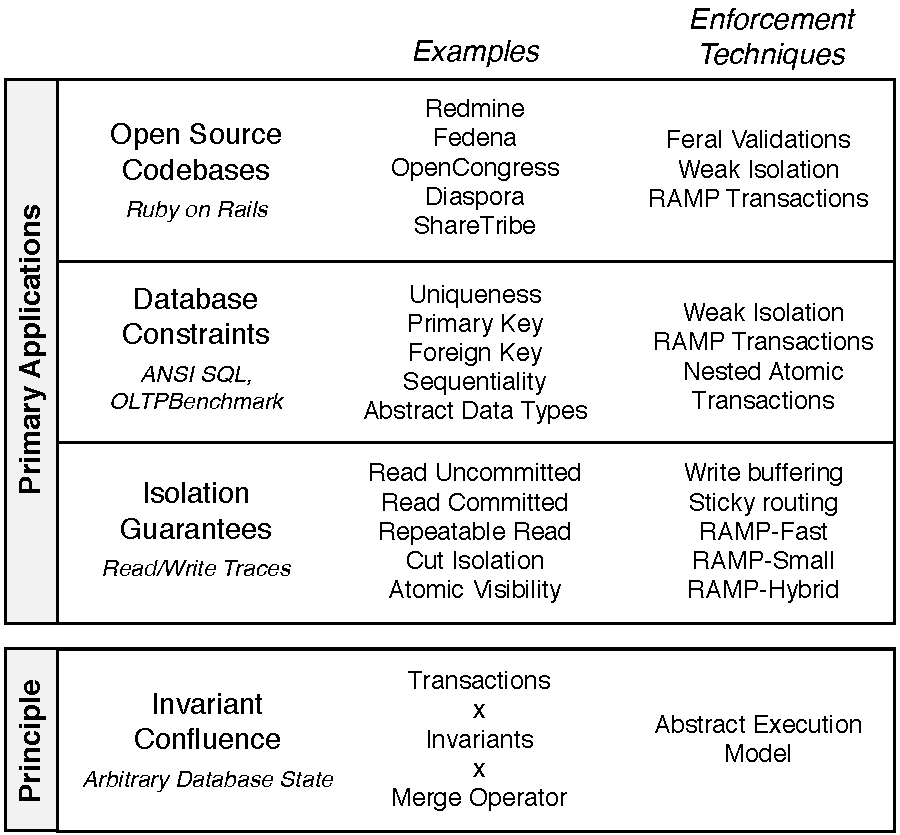
\includegraphics[width=\figscale\columnwidth]{diagram/contributions.pdf}
\vspace{.75em}
\caption{In this thesis, we develop the principle of \IConfluence, a
  necessary and sufficient condition for safe, convergent,
  coordination-free execution, and apply it to a range of application
  domains at increasing levels of abstraction: database isolation,
  database constraints, and safety properties from modern
  database-backed applications. Each guarantee that is \iconfluent is
  guaranteed to have at least one coordination-free implementation; we
  investigate the design of several implementations in this work,
  which operate at the database infrastructure tier (Figure~\ref{fig:servers}).}
\label{fig:contribs}
\end{figure}


In this section, we summarize the primary contributions of this work.

\newcommand{\contribution}[1]{\vspace{.5em}\noindent\textbf{#1}.\xspace\xspace}
%\begin{itemize}[label={}]
 \contribution{Coordination-free execution and \IConfluence}  We identify coordination-free execution as fundamental to available,
 low latency, and scalable system execution. To do so, we present a
 system model and show a direct correspondence between these desirable
 system properties and the ability to guarantee non-trivial progress
 in an asynchronous network.

 We subsequently develop the \iconfluence property, a necessary and
 sufficient condition for ensuring that a safety guarantee can be
 guaranteed under coordination-free, convergent execution of a given
 set of transactions. This is the first necessary and sufficient
 condition for these properties that we have encountered. In effect,
 \iconfluence lifts traditional partitioning arguments from
 distributed systems from the domain of event traces to the domain of
 arbitrary application logic and constraints over data. We use this
 property to examine and optimize a range of semantics from database
 systems (Figure~\ref{fig:contribs}), which we describe in turn below.

 \contribution{Coordination-free Isolation Guarantees} While
 transactional guarantees are often associated with serializability
 and its necessarily coordinated implementations, most databases in
 practice provide weaker forms of transactional isolation, or variants
 of admissible read-write interleavings (Figure~\ref{fig:contribs}).
 In a survey of 18 ``ACID'' and ``NewSQL'' databases, we find that
 only three offered serializability by default and only nine offered
 it as as an option at all. We investigate the weaker models offered
 by these databases and show that many are \iconfluent. For example,
 common isolation models such as Read Committed (default in eight
 databases) and ANSI Repeatable Read isolation are \iconfluent. Many
 guarantees, like Read Committed, arbitrated \textit{visibility} but
 not concurrency (much like causal consistency). The resulting
 taxonomy is one of the first unified treatments of weak isolation,
 distributed register consistency, session guarantees, and
 coordination requirements in the literature. Using these results, we
 implement a coordination-free prototype implementing weak isolation
 guarantees that achieves up to two order-of-magnitude latency
 reductions when deployed across datacenters.

  In addition to investigating existing isolation guarantees, we
  examine new guarantees. A number of applications leverage
  database-provided functionality for enforcing referential integrity,
  secondary indexing, and multi-get and multi-put operations, yet
  there is no coordination-free mechanism for enforcing
  them. Accordingly, a number of practitioner reports on systems
  (e.g., from Facebook, Google, LinkedIn, and Yahoo!) specifically
  highlight these use cases as scenarios where, lacking a
  coordination-free algorithm, architects explicitly sacrificed
  correctness for latency and availability. In response, we develop a
  new, \iconfluent isolation model called Read Atomic (RA) isolation 
  and set of scalable, coordination-free algorithms called Read Atomic
  Multi-Partition (RAMP) Transactions for addressing the isolation
  requirements of these use cases. Informally, RA guarantees
  \textit{atomic visibility} of updates: once one write from a
  transaction is visible, all writes will be visible. Existing
  protocols for achieving RA isolation (or stronger), such as distributed
  locking, couple atomic visibility with mutual exclusion; RAMP
  achieves the former without the cost of the latter. RAMP uses
  limited multi-versioning to allow clients to operate concurrently
  over the same data items while ensuring that readers can correctly
  detect and repair incomplete writes. Across a range of workloads
  (including high contention scenarios), RAMP transactions incur
  limited overhead and outperform existing mechanisms for achieving RA isolation
  while scaling linearly.

  \contribution{Coordination-free Database Constraints and Application
    Criteria} Moving from read-write traces to higher-level semantic
  properties (Figure~\ref{fig:contribs}), we examine the integrity
  constraints and invariants offered by databases today---including
  the foreign key constraints addressed by RAMP but also row-level
  check constraints, uniqueness constraints, and constraints on
  abstract data types---and classify each as \iconfluent or not. Many
  are \iconfluent, so we subsequently apply this classification to a
  number of database workloads from the OLTPBenchmark
  suite~\cite{oltpbench}. Many invariants in these workloads pass the
  \iconfluence test as well. For example, in the TPC-C benchmark, the
  gold standard for transaction processing performance, ten of twelve
  invariants are \iconfluent under the workload. Given this
  classification, we develop a database prototype and
  coordination-avoiding execution strategy for TPC-C that, on a
  cluster of 200 servers, achieves a 25-fold improvement in throughput
  over the prior best result (over 12.7M New-Order transactions per
  second).

  While we are able to find \iconfluent database integrity constraints
  and benchmarks, are \textit{real} applications \iconfluent?
  Moreover, are invariants a practical choice of correctness criteria?
  To answer these questions, we examine open source web applications
  to inspect their safety properties (Figure~\ref{fig:contribs}). We
  find that popular web programming frameworks---including Ruby on
  Rails, Django, and Spring/Hibernate---have introduced support for
  \textit{validations}, or declarative, application-level
  invariants. We subsequently analyze the use of validations in 67 of
  the most popular Ruby on Rails applications on GitHub and find that,
  in fact, validation usage is fourteen times more common than the use
  of database transactions. Moreover, more than 86.9\% (of over 9900
  invariants) are \iconfluent. However, the remainder are \textit{not}
  \iconfluent and therefore require coordination. For these
  invariants, we profile the incidence of constraint violations both
  with and without validations. In addition to demonstrating the
  applicability of \iconfluence, this study exposes a surprising
  practitioner trend away from transactions towards using invariants via
  validations.\vspace{.5em}

  In all, these results highlight a widespread potential for
  coordination-avoiding database system design within both classic and
  emerging database-backed applications. While coordination cannot
  always be avoided, in many common scenarios, we find it is possible to
  guarantee application safety within the database while also
  providing coordination-free execution. Our resulting database system
  prototypes and their regular order-of-magnitude speedups compared to
  conventional approaches evidence the power of this latent potential
  for coordination-avoiding execution.

\begin{comment}
   In addition to the above, we present a summary of additional results
  developed during our investigation of coordination avoidance,
  including: PBS, a new methodology for profiling the incidence of
  isolation violations in weakly consistent stores; the Bolt-on
  Architecture for upgrading the isolation of underlying eventually
  consistent data stores as well as an implementation of bolt-on
  causal consistency; Explicit Causality, an API for reducing the
  overheads of causal information tracking; and early results from
  applying coordination-avoiding execution to the tasks of distributed
  convex optimization and model serving and maintenance.
\end{comment}

\section{Outline and Previously Published Work}

The remainder of this dissertation proceeds as
follows. Chapter~\ref{c.background} provides background on
coordination and defines our system model. Chapter~\ref{c.iconfluence}
presents the \IConfluence
property. Chapters~\ref{c.isolation},~\ref{c.ramp},and~\ref{c.constraints}
examine the coordination requirements and coordination-free
implementations of transaction isolation, database functionality such
as indexes, and constraints. Chapter~\ref{c.relatedwork} discusses
related work and Chapter~\ref{c.conclusion} concludes with a
discussion of lessons learned, topics for future work, and closing
thoughts.

Chapter~\ref{c.background} includes material from several previous
publications~\cite{hat-vldb,coord-avoid,partitions-queue14,queue,pbs,pbs-vldbj2013,pbs-demo-sigmod2013}. Chapter~\ref{c.iconfluence}
revises material from~\cite{coord-avoid}. Chapter~\ref{c.isolation}
revises~\cite{hat-vldb} and~\cite{hat-hotos}. Chapter~\ref{c.ramp}
revises~\cite{ramp-sigmod14} and includes material
from~\cite{explicit-socc}. Chapter~\ref{c.constraints} revises
material from~\cite{coord-avoid} and~\cite{apps} and includes material
from~\cite{bolton}. Chapter~\ref{c.conclusion} includes material
from~\cite{velox-overview,admm}.


\begin{comment}
\section{Note on Exposition}

The goal of this thesis is the improved design of modern distributed
database systems. In doing so, we pursue a principled approach to
systems design that provides rigorous rationale for
\textit{why} a given system design is preferable (or at least
outperforms existing systems along some dimension, whether latency,
scalability, availability, or throughput); in this thesis, our primary
guiding principle is the pursuit of coordination-free execution. To
assist in this pursuit of principle, we adopt a modest amount of
formalism for the analysis of both semantics and our proposed
algorithms. Thus, while our ultimate objectives lie in the realm of
systems, we leverage machinery from more formal domains.

In our exposition, we have largely opted to present the systems
rationale and explanations first, followed by their respective
formalization and more rigorous treatment. To keep each chapter
self-contained, we have included the more formal components in the
body of each chapter (i.e., instead of in an appendix). However, we
have delineated each more formal section with an appropriate
heading. Readers with a more practical inclination may wish to skip
these sections upon first reading. Readers with a more formal
inclination may wish to pursue an alternative section ordering than we
have chosen here. Any ambiguities in the less formal prose should be
resolvable by consulting the more formal text.
\end{comment}